%!TEX root = paper.tex
\section{InferSpark Overview}
\label{sec:framework}

\begin{figure*}[th]
\centering
    \includegraphics[width=0.8\linewidth]{figs/workflow_future.eps}
    \caption{InferSpark Architecture}
    \label{fig:workflow}
\end{figure*}

%\begin{figure*}[th]
%	\centering
%	\includegraphics[width=1.6\columnwidth]{figs/workflow2.eps}
%	\caption{InferSpark Architecture}
%	\label{fig:workflow}
%\end{figure*}

%\KZ{My general feeling is that the running example is not made full use of.
%The discussion should be tightly coupled to the running example. E.g., when
%we talk about schedule, just present the schedule for the two coins.
%Some of the stuff here should go into implementation section.}

The overall architecture of InferSpark is shown in \figref{fig:workflow}.  An
InferSpark program is a mix of Bayesian network model definition and normal
user code. The Bayesian network construction module separates the model part
out, and transforms it into a Bayesian network template. The algorithm
matching module selects the applicable inference algorithm (e.g. variational
message passing). The template is
then instantiated with parameters and metadata from the input data at runtime
by the code generation module, which produces the inference code. These are
then executed on the Spark distributed engine to produce the final posterior
distribution.

%Note that we currently hard-code the VMP algorithm into CodeGen module of
%InferSpark, which only supports certain exponential-conjugate Bayesian
%networks. We plan to implement other inference algorithms such as Belief
%Propagation, Gibbs Sampling, etc. to handle other common types of Bayesian
%networks.

%InferSpark analyzes the Bayesian network defined by a special 
%scala-like program and
%automatically transforms the model definition into the GraphX implementation
%of VMP algorithm. After two stages of compilation, the runtime system 
%launches the VMP implementation and returns the inference results 
%through the query API.  
Next, we describe the key modules in more details with the help of
some Baysian models. 
%the example of the two-coin model (\figref{fig:two_coin_bn}). 

\subsection{Running Examples}

\KZ{Four running examples:}
\begin{itemize}
\item TwoCoin
\item SLDA
\item GMM
\item Bayes Point Machine
\end{itemize}

\KZ{Give the InferSpark definition of the four examples.
}


\begin{figure}[h]
\begin{lstlisting}
@Model class TwoCoins(alpha: Double, beta: Double) {
	val pi = Beta(alpha)
	val phi = (0L until 2L).map(_ => Beta(beta))
	val z = ?.map(_ => Categorical(pi))
	val x = z.map(z => Categorical(phi(z)))
}
object Main {
	def main() {
		val xdata: RDD[Long] = /* load (observed) data */
		val m = new TwoCoins(1.0, 1.0)
		m.x.observe(xdata)
		m.infer(steps=20)
		val postPhi: VertexRDD[BetaResult] = m.phi.getResult()
		/* postprocess */
		...
	}
}
\end{lstlisting}
\caption{Definition of two-coin model in InferSpark}
\label{fig:two_coins_modeldef}
\end{figure}

%Apart from ordinary scala code, the input program of InferSpark contains the
%statistical model definitions. The syntax of the model definition extends
%from the scala syntax.  
\figref{fig:two_coins_modeldef} shows the definition of the two-coin model
in InferSpark. The definition starts with ``{\sf @Model}'' annotation. 
The rest is similar to a class definition in
scala. The model parameters (``{\sf alpha}'' and ``{\sf beta}'') are constants to the
model. In the model body, only a sequence of value definitions are allowed,
each defining a random variable instead of a normal deterministic variable. 
The use of ``{\sf val}'' instead of ``{\sf var}'' in the syntax 
implies the conditional dependencies between random variables are fixed 
once defined. For example, line
2 defines the random variable $\pi$ having a symmetric Beta prior
$\mathrm{Beta}(\alpha, \alpha)$.

InferSpark model uses ``Range'' class in Scala to represent plates. Line 3
defines a plate of size 2 with the probabilities of seeing head in the 
two coins. The ``?'' is a special type of ``Range'' representing 
a plate of unknown size at the time of model definition. 
In this case, the exact size of the plate will be provided or inferred
from observed variables at run time.  When a random variable is
defined by mapping from a plate of other random variables, 
the new random variable is in the same plate as the others.  
For example, line 5 defines the outcomes $x$ as the mapping from $z$ 
to Categorical mixtures, therefore $x$ will be in the same plate as
$z$. Since the size of the plate surrounding $x$ and $z$ is unknown, we need
to specify the size at run time.  We can either explicitly set the length of
the ``?'' or let InferSpark set that based on the number of observed outcomes
$x$ (line 11).

At the first glance, ``?'' seems redundant since it can be replaced by a
model parameter $N$ denoting the size of the plate.  However, ``?'' becomes
more useful when there are nested plates. In the two-coin model, suppose
after we choose one coin, we toss it multiple times. 
\figref{fig:two_coins_nestedplates} shows this scenario.
Then the outcomes $x$ are in two nested plates where the inner plate is
repeated $M$ times, and each instance may have
a different size $N_i$. Using the ``?'' syntax
for the inner plate, we simply change line 5 to

{\small\begin{verbatim}
	val x = z.map(z => ?.map(_ => Categorical(phi(z))))	
\end{verbatim}
}

\begin{figure}[th]
	\centering
	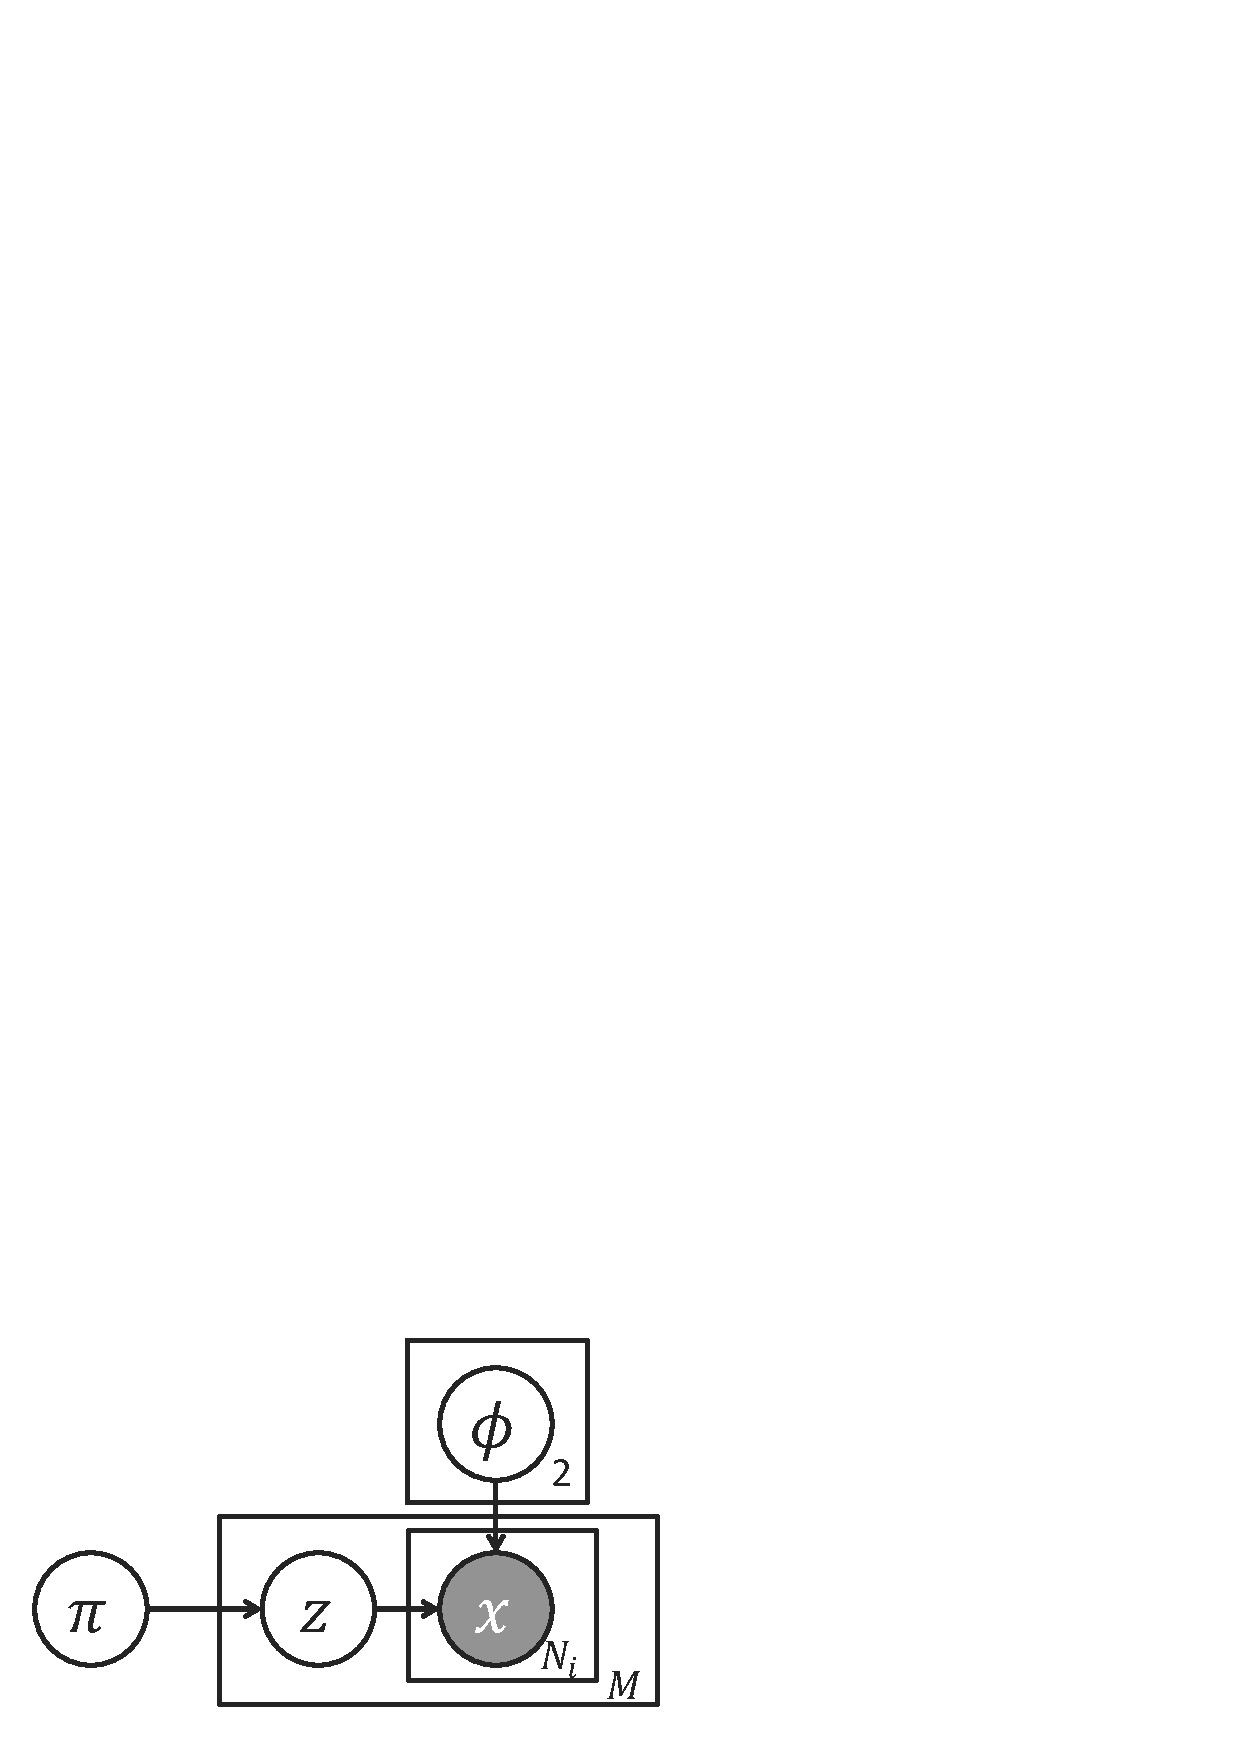
\includegraphics[width=0.25\textwidth]{figs/two_coins_nestedplates}
	\caption{Two-coin Model with Nested Plates}
	\label{fig:two_coins_nestedplates}
\end{figure}

\subsection{Bayesian Network Construction}

\begin{figure}[h]
\centering
\includegraphics[scale=0.4]{figs/two_coins_bn1.eps}
\caption{Bayesian Network Template Constructed from the Two-coin Model}
\label{fig:two_coins_bn1}
\end{figure}

An input InferSpark program is first parsed and separated into two parts: 
the model definition (``{\sf @Model} class TwoCoins'' in 
\figref{fig:two_coins_modeldef}) and
the ordinary scala program (``{\sf object Main}'' in
\figref{fig:two_coins_modeldef}). The model definition is analyzed and
transformed into valid scala classes that define a Bayesian
network constructed from the model definition 
(e.g., \figref{fig:two_coins_bn1}) and the inference/query API.
Note the Bayesian network
constructed at this stage is only a template (different than 
\figref{fig:two_coin_bn}) because some of the information is not available 
until run time (e.g., the outcomes $x$, the number of coin flippings 
and the model parameters $\alpha$ and $\beta$). 
%A snippet of generated two-coin code (with simplified variable names)
%is shown in \figref{fig:two_coins_stage1code}.
%
%\begin{figure}[h]
%\centering
%\begin{lstlisting}
%class TwoCoins(alpha: Double, beta: Double) extends ModelBase {
%	val synval$internal$parent: Array[Int] = /**/
%	var Categorical$13$isObserved: Boolean = _
%	class Categorical$13$Inferface extends RandomVariable {
%		def observe(obs: RDD[Long]) = /* ... */
%		def getResult(): RDD[CategoricalResult] = /* ... */
%	}
%	val x = new Categorical$13$Interface()
%	/* ... */
%}
%\end{lstlisting}
%\caption{Bayesian Network Code}
%\label{fig:two_coins_stage1code}
%\end{figure}
%
%The Bayesian network source code is then compiled with the
%ordinary scala program into bytecode. This bytecode will generate the
%inference code of the VMP algorithm for the model on GraphX in
%the next 4 steps.
%
%The InferSpark model definition is a scala definition with ``@Model''
%annotation. The scala parser first separates the model definition from other
%part of the program (i.e. user program). A Bayesian network is then constructed
%according to dependencies between the random variables in the model definition.
%\figref{fig:lda_bn1} is the Bayesian network constructed from the LDA model
%definition. Some information only available at runtime are missing from the
%Bayesian network, e.g. the number of topics $K$, the observed words $w$, etc.
%At this step, the analyzer also verifies that the model is in the
%exponentail-conjugate family and rejects unsupported model definitions. After
%the construction, the Bayesian network is stored in the compiled program for
%later steps to process.

%\begin{figure}[!h] 
%	\centering 
%	\includegraphics[scale=0.3]{figs/lda_bn1.eps}
%	\caption{Bayesian Network Constructed From the Model Definition}
%	\label{fig:lda_bn1}
%\end{figure}

\subsection{Metadata Collection}

Metadata such as the observed values and the plate sizes missing from the
Bayesian networks are collected at runtime. In the two-coin
model, an instance of the model is created via the constructor invocation (e.g.
``{\sf val m = new TwoCoin(1.0, 1.0)}'' on line 10 of \figref{fig:two_coins_modeldef}). The constructor call provides
the missing constants in the prior distributions of $\pi$ and $\phi$. 
For each random variable defined in the model definition, 
there is an interface field with the
same name in the constructed object. Observed values are provided to InferSpark
by calling the ``{\sf observe}'' (line 11 of \figref{fig:two_coins_modeldef}) 
API on the field. 
There, the user provides an RDD of observed outcomes ``{\sf xdata}'' to InferSpark by calling
``{\sf m.x.observe(xdata)}''. The  {\sf observe} API also triggers 
the calculation of unknown plate sizes. 
In this case, the size of plate surrounding $z$ and $x$ is
automatically calculated by counting the number of elements in the RDD.

%When the user provide the observed random variables such as the words in the
%LDA model, the number of documents and the number of words in each document
%can be inferred from the data. This is different from most libraries in that
%they require the user to explicitly set the numbers or to transform the data
%into a library-specific format. InferSpark also tries to verify that the user
%have provided consistent data. For example, InferSpark will report an error,
%if the user provides data to both the topics $z$ and the words $w$ but they
%have differnt sizes.

\subsection{Algorithm Matching \& Code Generation}

\begin{figure}
\centering
	\includegraphics[width=0.35\textwidth]{figs/two_coins_msg.eps}
	\caption{Bayesian Network with Messages for Two-coin Model}
	\label{fig:two_coins_msg}
\end{figure}

When the user calls ``{\sf infer}'' API (line 12 of
\figref{fig:two_coins_modeldef}) on the model instance, InferSpark checks
whether all the missing metadata are collected. If so, it proceeds to
algorithm matching module. 
\KZ{Introduce three diff algos: VMP, Gibbs and EP. We might need to discuss 
the basic parallel version of these algos separately here.}
In this case, the module finds that the model is in
exponential-conjugate family so the VMP algorithm is applicable to it. The
Code Generation module then annotates the Bayesian network with messages used
in VMP, resulting in \figref{fig:two_coins_msg}. The expressions that
calculate the messages (e.g., $E_{Q_\pi}[\ln \pi]$) depend on not only the
structure of the Bayesian network and whether the vertices are observed or
not, but also practical consideration of efficiency and constraints on GraphX and Spark.

%The inference algorithm we use is the variational message passing algorithm.
%This step annotates the messages and vertex updates of the algorithm to the
%Bayesian network from previous step and we call the resuling graph as message
%passing graph.
%
%The VMP algorithm is expressed as sending messages of functions of sufficient
%statistics of random variables and updating the sufficient statistics by
%aggregating the messages. The messages are sent in both direction of the edges
%in the Bayesian network. The vertices are updated by aggregating incoming
%messages. For the Dirichlet random variables, the update is simply adding
%together all the messages. The unobserved Categorical random variable $z$ is
%updated by normalizing the sum of the messages. The observed Categorical
%mixtures $w$ have nothing to update but have to compute the new messages to $z$
%and $\phi$ according to the incoming messages.

%\begin{figure}[h]
%	\centering	
%	\includegraphics[scale=0.3]{figs/lda_mpg.eps}
%	\caption{Message Passing Graph of LDA}
%	\label{fig:lda_mpg}
%\end{figure}


%The messages in the VMP algorithm are sent in both directions. The messages
%along the edge only depend on the sender but the messages in the reverse
%direction may also depend on other parents' message.  For example, the message
%along the edge from $z$ to $w$ only depends on the sufficient statistics of
%the Categorical variable $z$, but the reverse one will depend on the
%topic-word distributions' messages. The original VMP algorithm assumes that
%only one vertex may be updated in each step and the messages that the vertex
%depends on are always up-to-date.  However, this poses two challenges when
%implementing it as a distributed message passing algorithm. First, we have to
%relax the assumption of one vertex in each step to increase parallelism
%without violating the correctness of the algorithm. In the LDA example,
%Updating all the random variables at the same time does not guarantee to
%optimize the ELBO but we can update all the topics at the same time because it
%is equivalent to sequentially update each of the topics. Secondly, vertecies
%that have not been updated could send messages that depends on stale messages.
%If updates to the topics $z$ are immediately followed by updates to the
%topic-word distributions $\phi$, the messages from $w$ to $\phi$ will depend
%on the messages sent from $z$ to $w$ prior to the update of $z$ instead of the
%new messages from $z$ to $w$. Therefore, we choose an update schedule that is
%equivalent to sequential updates to ensure the correctness of the algorithm.

%\subsection{MPG Construction Code Generation}
To convert the Bayesian network to a message passing graph on GraphX,
InferSpark needs to construct a VertexRDD and an EdgeRDD. This step generates
the MPG construction code specific to the data.
\figref{fig:two_coins_mpg_constr_code} shows the MPG construction code
generated for the two-coin model. 
The vertices are constructed by the union
of three RDD's, one of which from the data and the others from 
parallelized collections (lines 8 and line 9 in \figref{fig:two_coins_mpg_constr_code}).
The edges are built from the data only. 
A partition strategy specific to the
data is also generated in this step.




\begin{figure}[h]
\begin{lstlisting}
class TwoCoinsPS extends PartitionStrategy {
	override def getPartition /**/
}
def constrMPG() = {
	val v1 = Categorical$13$observedValue.mapPartitions{
		initialize z, x */
	}
	val v2 = sc.parallelize(0 until 2).map{ /* initialize phi */ }
	val v3 = sc.parallelize(0 until 1).map{ /* initialize pi */ }
	val e1 = Categorical$13$observedValue.mapParititons{
		/* initialize edges */
	}
	Graph(v1 ++ v2 ++ v3, e1).partitionBy(new TwoCoinsPS())
}
\end{lstlisting}
\caption{Generated MPG Construction Code}
\label{fig:two_coins_mpg_constr_code}
\end{figure}
%Constructing the
%message passing graph of the Bayesian network is not trivial because different
%types of random variables have different initialization methods and different
%data sources. The initialization of the outcomes $x$ in the two-coin model is
%fixing its distribution to a point categorical distribution at the observed
%outcome and randomly initialize the incoming messages while the initialization
%of the choice of coins $z$ is to randomly initialize the parameters of its
%approximate marginal posterior distribution. The data source of $x$ is the
%observed outcomes while $z$ does not have data source. The initialization of
%EdgeRDD is also nontrivial because the links between different random
%variables have different structures. Inferspark finds a transformation plan
%for the MPG construction. A possible plan for the two-coin model is shown in
%\figref{fig:two_coins_mpg_construction_plan}.
%
%\begin{figure}[h]
%	\centering
%	\includegraphics[width=0.45\textwidth]{figs/two_coins_mpg_construction_plan.eps}
%	\caption{MPG Construction Plan of Two-Coin Model}
%		\label{fig:two_coins_mpg_construction_plan}
%\end{figure}

%In a typical GraphX application, the property graph has homogeneous vertex
%properties and edge properties. In the shortest distance application, the
%vertex properties are shortest distance from the origin and edges properties
%are weights. The EM algorithm implementation for LDA in Mllib, which only
%computes the Maximum A Posterior rather than the full posterior, uses the
%vertex properties as topic counts and edge propertices as word counts. However,
%the message passing graph of the VMP algorithm generally have heterogeneous
%vertex properties and edge properties. In the LDA case, we have three types of
%vertecies: observed categorical mixture, unobserved categorical variable and
%unobserved dirichlet variable. The observed categorical mixture needs to store
%the messages from parents and the observed value while the other two types need
%to store the sufficient statistics. The edges also have differnt structures.
%There's one-to-one correspondence between $z$ and $w$ while $w$ are fully
%connected to $\phi$. Therefore, the compiler need to create an unrolling plan
%so that the graph is correctly initialized. In the LDA case, a possible plan is
%to first map from the observations of x to create vertecies for $\theta$, $z$
%and $x$ and use a parallelized range to create verticies for $\phi$. Another
%possibility is to separately initialize each set of variables.  We try to
%minimize the overhead of union by merging the initialization of variables as
%much as possible.

In addition to generating code to build the large message passing graph,
the codegen module also generates code for VMP iterative inference. 
InferSpark, which
distributes the computation, needs to create a schedule of parallel updates
that is equivalent to the original VMP algorithm, which only updates one vertex
in each iteration.  Different instances of the same random variables can be
updated at the same time. An example update schedule for the two-coins model is
($\pi$ and $\phi$) $\rightarrow$ $x$ $\rightarrow$ $z$ $\rightarrow$ $x$. VMP inference code that enforces the update
schedule is then generated. % \ERIC{how to derive this indeed?}

InferSpark currently include the VMP algorithm while other inference algorithms
such as Belief Propagation, Gibbs Sampling and etc. will be added to it in
order to support inference on a wider range of Bayesian networks. We will also
publish a high-level language for implementing inference algorithms and
specifying what models the algorithms apply to.  Algorithm developers are
welcomed to add new algorithms whenever existing ones do not fit the needs of
end-users. Algorithm matching module searches for an applicable algorithm among
both the built-in and the developer-suppied inference algorithms while the new
CodeGen module transforms the algorithm into a Spark program and handles all
the low-level optimizations. These two modules are similar to efforts like
SystemML, MLI, which targets algorithm developers, but an integrated part of
InferSpark.

\subsection{Getting the Results}
%InferSpark finally compiles the VMP algorithm into a separate GraphX
%program and submit it to the Spark master. The user can specify how many
%iterations to run. 
The inference results can be queried through the ``{\sf getResult}''
API on fields in the model instance that retrieves a VertexRDD of approximate
marginal posterior distribution of the corresponding random variable. For
example, in Line 13 of \figref{fig:two_coins_modeldef}, ``{\sf m.phi.getResult()}'' 
returns a VertexRDD of two Dirichlet distributions. 
The user can also call ``{\sf lowerBound}'' 
on the model instance to get the evidence lower bound (ELBO) of the result, 
which is higher when the KL divergence between the approximate posterior 
distribution and the true posterior is smaller. 

\begin{figure}[h]
\centering
\begin{lstlisting}
var lastL: Double = 0
m.infer(20, { m =>
	if ((m.roundNo > 1) || 
		(Math.abs(m.lowerBound - lastL) < 
		   Math.abs(0.001 * lastL))) {
		false
	} else {
		lastL = m.lowerBound
		true	
	}
})
\end{lstlisting}
\caption{Using Callback function in ``infer'' API}
\label{fig:two_coins_callback}
\end{figure}

The user can also provide a callback function that will be called after
initialization and each iteration. In the function, the user can write
progress reporting code based on the inference result so far. 
For example, this function may return {\em false} whenever
the ELBO improvement is smaller than a threshold 
(see \figref{fig:two_coins_callback}) indicating the result is good enough 
and the inference should be terminated. 

%With all the information collected and calculated in previous steps,
%implementation of the inference algorithm as a GraphX program is generated,
%compiled and then executed. User can retrieve the posterior distributions as
%VertexRDDs through API calls.

